\documentclass[11pt, twocolumn]{article}

\usepackage{booktabs}
\usepackage[table,xcdraw]{xcolor}

\usepackage{bnaic}
\usepackage[ruled,vlined]{algorithm2e}
\usepackage{graphicx}
\usepackage{caption}
\usepackage{subcaption}
\usepackage{adjustbox}
\usepackage{pdflscape}
\usepackage{float}
\usepackage{hyperref}
\usepackage{lipsum}
\usepackage{comment}
\usepackage{iftex}
\usepackage{todonotes}
\usepackage{amsmath}

% Uncomment next two lines to disable figures (helps to see report length)
%\usepackage[figuresonly,nolists,nomarkers]{endfloat}
%\renewcommand{\processdelayedfloats}{}

\usepackage{fancyhdr}
\fancypagestyle{firstpage}
{
    \renewcommand{\headrulewidth}{0pt}
    \setlength{\headheight}{60pt} 
    \fancyhead[C]{
\includegraphics[width=14.5cm]{header/logo_rug_fse_ai.png}}
}


% \title{
\includegraphics[width=14.5cm]{header/logo_rug_fse_ai.png}\\\vspace{2cm}\textbf{\scshape{Bach Ex Machina}}}
\title{\vspace{1.5cm}\textbf{\scshape{Bach Ex Machina}}}
\author{
    Jorn van Wier\\
    \small j.h.a.van.wier@student.rug.nl
    
    \and 
    
    Ruurd Bijlsma\\
    \small r.bijlsma.3@student.rug.nl
    
    \and 
    
    Nischal Madiraju\\
    \small n.madiraju@student.rug.nl
    
    \and 
    
    Pranav Vallala\\
    \small p.g.vallala@student.rug.nl
}
\date{February 2021}

\pagestyle{plain}

\begin{document}

% \begin{figure*}[ht]
%     \centering
%     
\includegraphics[width=14.5cm]{header/logo_rug_fse_ai.png}
% \end{figure*}

\maketitle

\thispagestyle{firstpage}

\begin{abstract}
\noindent
The Art of the Fugue is Johann Sebastian Bach's incomplete musical work written in the last decade of his life. In this project, we are using multivariate LSTM and the MAESTRO dataset (V3.0.0) to generate pseudo-Bach music that can serve as a part of Bach's unfinished fugue. 
In training our model we try to determine the optimal loss function, optimizer and other hyperparameters. However, it's very difficult to create a loss function that is able to determine whether the generated music sounds 'good'. Therefore, for our final result, we evaluate the sound manually to determine how well the model performed.

Our final LSTM network is able to produce piano music after training on Bach's compositions, we used this ability to generate an ending to Bach's unfinished fugue. \ifpdf
In this report we show the findings visually, there is also an interactive version of this report where the reader can listen to the produced audio. This interactive version can be found at \url{https://ruurdbijlsma.github.io/bach-ex-machina/}.
\fi

\end{abstract}
\section{Introduction}
An interesting new application of the advances in the machine learning world is the artificial music generation. The ML models don't require explicit training by a human with extensive knowledge of music and its composition. The models pick up on patterns of harmony and learn on their own. 

In this paper, we use this methodology of artificial music generation for completing the unfinished composition of Johann Sebastian Bach, "The Art of the Fugue". We are using time-series based models to learn the respective patterns and generate a continuation of the unfinished composition. 
\subsection{Problem}
% Jorn
In 1993, a time series prediction competition the Santa Fe Institute organized a time series prediction competition. One of the tasks for this competition was to complete a fugue by Johann Sebastian Bach, which was left unfinished as he died before completing his work. 
An analysis of the data for this task can be found in \cite{dirstt1993baroque}. In our work, we use an LSTM model to perform the same task. As deep learning techniques such as LSTM models benefit greatly from more input data, a richer dataset than the one for the Santa Fe competition would be very valuable.

\subsection{Dataset}
% Ruurd
To train our network we use the MAESTRO v3 dataset \cite{hawthorne2018enabling}. This dataset is composed of over 200 hours of piano performances captured with fine alignment ($\sim$3ms) between note labels and audio waveforms. The data consists of MIDI files recorded by a Yamaha Disklavier, a concert-quality acoustic grand piano. 
\par
The train/test split is provided by the authors of the dataset, this split is configured in a way such that the same composition does not appear in multiple subsets. The music in the dataset is mostly classical, including music composed from the 17th to early 20th century.

\subsubsection{MIDI}
Our music generation method is based around MIDI files. MIDI files provide a compact and real-world representation of instrumental audio, which makes them useful for our training purposes. A MIDI file can consist of one or more tracks. For example, Bach's unfinished fugue has four tracks. Each of these tracks contains messages, specifying events such as a piano key being pressed or released, or a piano foot paddle being pressed. A message consists of metadata such as velocity, pitch, and precise timing. In the case of a piano, the velocity indicates how hard a key was pressed. 
\par
For our model, we transform the MIDI files to a simpler format. The entire MIDI file is converted to a 2D array with the pitch on one axis, and time on the other axis. This representation is visualized in \autoref{fig:represent}. In MIDI, the pitch is always an integer value between 0 and 128 (exclusive), therefore the size of the 2D array representation is always 128 x time units, time units being the length of the MIDI in ticks.
\begin{figure*}
    \centering
    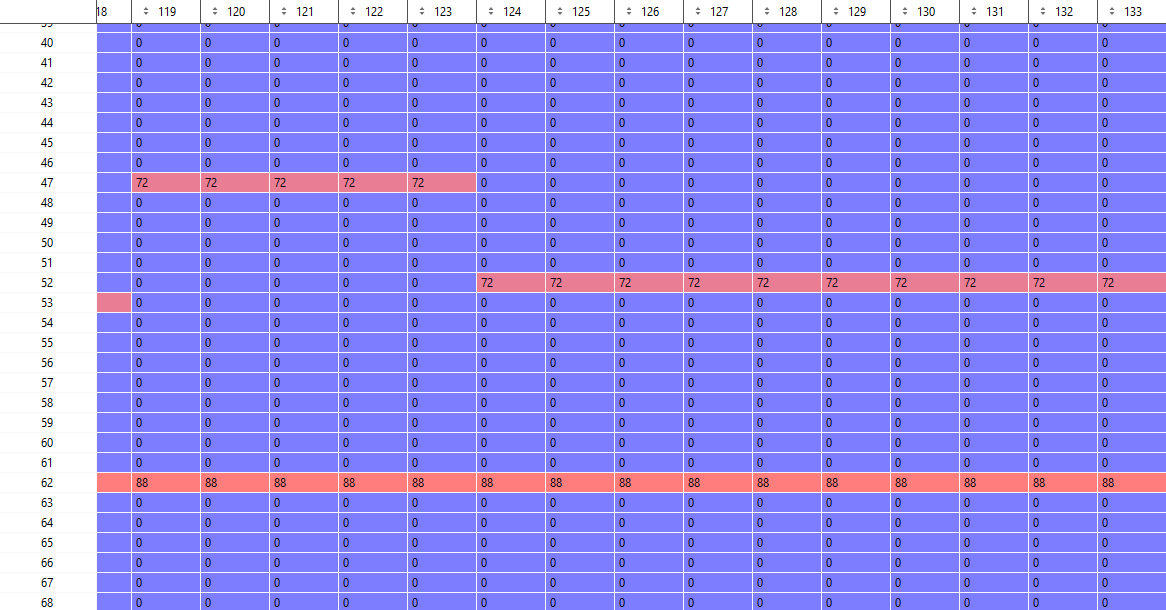
\includegraphics[width=\textwidth]{images/data.png}
    \caption{Example of a slice of the transformed MIDI file. The y-axis represents pitch, the x-axis represents time in ticks.}
    \label{fig:represent}
\end{figure*}
\par
The time units (ticks) used in MIDI are based on the tempo, which can change through each track, and a value called ticks per beat which is a constant value for each MIDI file. In our representation we simplify this by using our own ticks which always represent the same time unit (1/8th of a second) and assigning a velocity in the 2d array when at the timestamp a note was pressed at that level of pitch. For example, in \autoref{fig:represent}, a key was pressed for five ticks (from tick 119 to 123) with a pitch of 47, with a velocity of 72.
By using this representation we merge all tracks present in the MIDI file into one format, therefore we support MIDI tracks with any number of tracks.

Once we have transformed a MIDI file to this format, we can feed it into a number of machine learning models, such as a hidden Markov model or an LSTM network. Such models should then output in the same format, so that we can convert the predicted values back to a MIDI file, which can be played by a synthesizer (or a computer).

To reduce the dimensions of the input and output of the models we strip the 2D input array of all rows where there are no notes being pressed. In the Bach set of MIDI files from the Maestro dataset, this reduces the number of possible notes to 85, from 128. A visualization of the unfinished fugue can be seen in \autoref{fig:input_samples}.


\begin{figure}
    \centering
    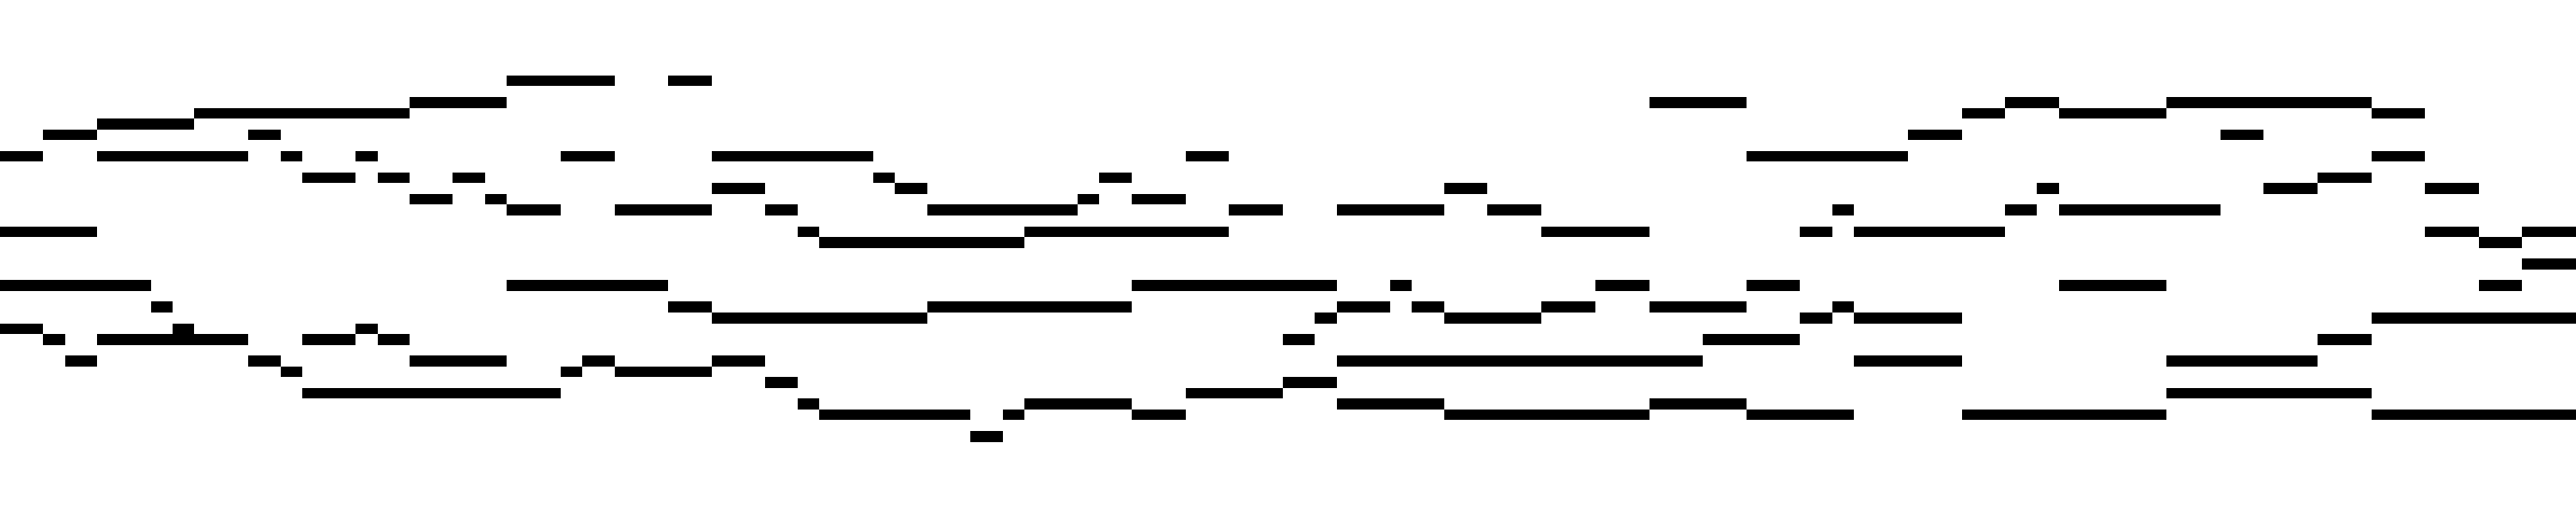
\includegraphics[width=\linewidth]{images/unfin_array.png}
    \caption{The unfinished fugue represented in our 2D format. The vertical axis represents pitch, the horizontal axis represents time.}
    \label{fig:input_samples}
\end{figure}
    
\subsection{Objectives}
Our main objective for this project is to create a model capable of autonomously generating the ending of a given classical song that's played on a piano. Besides the model we want to create software making the process of generating the ending of a song relatively easy to do.

\section{Baseline Model}
To help determine the success of our final LSTM model, we will compare it to a non-deep learning based model, namely a hidden Markov Model. We use a Gaussian hidden Markov model and train it on only one input song, Bach's unfinished fugue. The velocity values of the simplified representation are not used in this model, as this leads to more chaotic, less musical sounding results. By only feeding the model a 1 for a note pressed and 0 for silence, we can threshold the output of the model and tune it to audibly produce better results.

\begin{figure}
    \centering
    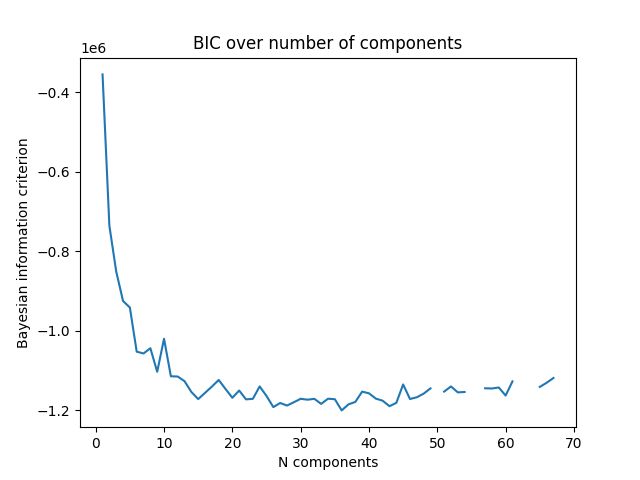
\includegraphics[width=\linewidth]{images/hmm_unfin_bic.png}
    \caption{BIC score per $N$ states for the hidden Markov model (lower score is better).}
    \label{fig:bic}
\end{figure}

We use a diagonal covariance type for this model. Since we do not know how many states there should be in this hidden Markov model, we calculated the Bayesian information criterion for a model train with every number of states from 1 to 70. The lowest scoring model is the model we used. The score for every number of states can be seen in \autoref{fig:bic}. The best model was found at 36 states.

The predicted samples from this model were thresholded to produce ones and zeroes. This thresholded 2D array was then converted to a MIDI file, and an image visualizing these notes. 

\section{LSTM}
For our project, we chose to use the LSTM architecture. LSTM stands for Long Short-Term Memory and is an architecture of Recurrent Neural Networks (RNNs). Previously, LSTM models have been used to great success in machine translation \cite{googleLSTMtranslation}, music composition \cite{Eck02learningthe} and time series anomaly detection \cite{malhotra2015long}.

An LSTM unit consists of a cell and a number of gates. The cell is what stores the state of the unit (memory), and the gates control the flow of information into and out of the unit. Originally, there were two gates, the input gate and the output gate. Later, the forget gate (or keep gate) was introduced, enabling the LSTM to forget the state in its cell \cite{LSTMSearchSpaceOdyssey}.

\subsection{Model architecture}\label{architecture}
% Ruurd
% Explain hyper parameters
% Epochs
The architecture of our final model is shown in \autoref{fig:arch}. The starting premise for our architecture was to have an LSTM layer and a fully connected layer with the number of possible notes as the output size. We found that this model was not able to really learn the structure of the music. This model performed with about 1.1\% accuracy, meaning it essentially put out random notes (88 possible notes, 1/88 is approximately 0.011). To try to improve the model, we increased the depth of it. We added two more fully connected layers, another LSTM layer and a 1D convolutional layer at the start. Using the SGD optimizer, we measured an accuracy of ~27\% on the test data. We named this architecture "medium", it has 73,302 parameters.

\begin{figure}
    \centering
    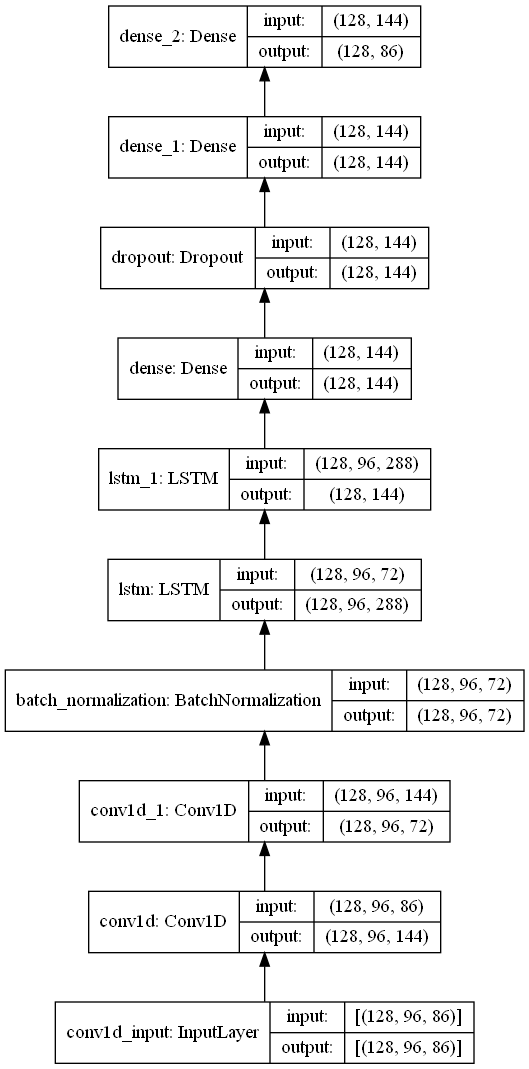
\includegraphics[width=\linewidth]{images/big.png}
    \caption{Visualization of the architecture of the most accurate model (named "big").}
    \label{fig:arch}
\end{figure}

From this point, we iterated on the architecture and the hyperparameters by measuring the test accuracy for each configuration after training for either 25 epochs, or until the validation loss stops improving. We created some variations on the model architecture, namely, a smaller and a bigger version of it. The small version removes one of the fully connected layers and halves the amount of nodes per layer. This "small" network has 19,414 parameters. The big version adds another 1D convolutional layer and increases the number of nodes per layer by a factor of about 2 to 4. This "big" network has 827,726 parameters.

\begin{table*}
    \centering
    \begin{tabular}{@{}llllrr@{}}
        \toprule
        \textbf{Network}               & \textbf{Loss}                               & \textbf{Optimizer}            & \textbf{Activation}             & \multicolumn{1}{l}{\textbf{Window size}}                                & \multicolumn{1}{l}{\textbf{Accuracy (\%)}} \\ \midrule
        big                            & categorical cross-entropy                    & SGD                           & Sigmoid                         & \multicolumn{1}{r|}{96}                                                 & \textbf{28.3}                              \\
        big                            & categorical cross-entropy                    & \cellcolor[HTML]{9AFF99}Nadam & Sigmoid                         & \multicolumn{1}{r|}{96}                                                 & \textbf{32.2}                              \\
        big                            & \cellcolor[HTML]{FFCCC9}binary cross-entropy & Nadam                         & Sigmoid                         & \multicolumn{1}{r|}{96}                                                 & \textbf{27.3}                              \\
        big                            & \cellcolor[HTML]{FFCCC9}mean squared error  & Nadam                         & Sigmoid                         & \multicolumn{1}{r|}{96}                                                 & \textbf{25.4}                              \\
        \cellcolor[HTML]{FFCCC9}medium & mean squared error                          & Nadam                         & Sigmoid                         & \multicolumn{1}{r|}{96}                                                 & \textbf{22.9}                              \\
        big                            & categorical cross-entropy                    & Nadam                         & \cellcolor[HTML]{FFCCC9}Softmax & \multicolumn{1}{r|}{96}                                                 & \textbf{0.9}                               \\
        \cellcolor[HTML]{FFCCC9}medium & categorical cross-entropy                    & Nadam                         & Sigmoid                         & \multicolumn{1}{r|}{96}                                                 & \textbf{30.3}                              \\
        \cellcolor[HTML]{FFCCC9}medium & categorical cross-entropy                    & Nadam                         & Sigmoid                         & \multicolumn{1}{r|}{\cellcolor[HTML]{FFCCC9}64}                         & \textbf{31.0}                              \\
        big                            & categorical cross-entropy                    & Nadam                         & Sigmoid                         & \multicolumn{1}{r|}{\cellcolor[HTML]{9AFF99}128}                        & \textbf{32.7}                              \\
        \cellcolor[HTML]{FFCCC9}small  & categorical cross-entropy                    & Nadam                         & Sigmoid                         & \multicolumn{1}{r|}{96}                                                 & \textbf{27.1}                              \\
        big                            & categorical cross-entropy                    & \cellcolor[HTML]{FFCCC9}Adam  & Sigmoid                         & \multicolumn{1}{r|}{\cellcolor[HTML]{FFFFFF}{\color[HTML]{000000} 128}} & \textbf{29.2}                              \\
        \bottomrule
    \end{tabular}
    \caption{Testing results of different training configurations. Accuracy measures test accuracy after 25 epochs or after the validation loss stops improving. Activation refers only to the activation of the output layer. Highlighted cells are changes from previous best configuration. }
    \label{tab:results}
\end{table*}

The results from our testing can be seen in \autoref{tab:results}. This table shows our best configuration having 32.7\% accuracy. In the best configuration we use the "big" architecture, shown in \autoref{fig:arch}. A larger network seems needed to properly learn from our input, which is relatively complex. 

\subsubsection{Loss function}
Our dataset can contain multiple notes per time unit, meaning we need a loss function that is compatible with multi-label output. Our output is either 1 or 0, which determines if a note should be played at that time step and at that pitch.
Initially, we used binary cross-entropy, because it is traditionally used for this sort of problem. However, we found that this resulted in lower performance than categorical cross-entropy. While this is counter-intuitive given the multi-label data, these findings are similar to observations in \cite{Mahajan_2018_ECCV}. Mean squared error was also tested: this loss function caused the network to converge much slower, but it did eventually achieve 22.9\% accuracy.

\subsubsection{Optimizer}
The optimizers that we tested are SGD with Nesterov momentum, Nadam and Adam. Using Nadam resulted in the largest testing accuracy, so this is the optimizer we used for our final model.

\subsubsection{Window size}
The window size determines how far back the LSTM gets data from relative to the current time step. A larger window size can mean the LSTM can learn longer dependencies and therefore lead to a more accurate network.

\subsection{Training}
Training was done for 25 epochs, or until the validation loss stopped improving. The loss over epochs and accuracy are plotted in \autoref{fig:loss} and \autoref{fig:acc}.
\begin{figure}
    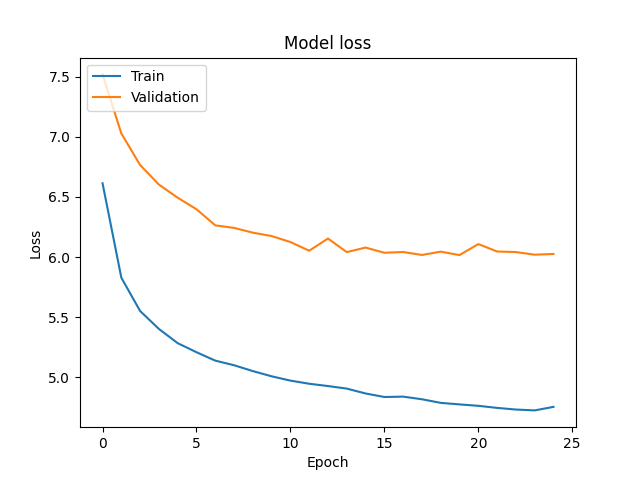
\includegraphics[width=\linewidth]{images/loss_bach_big_categorical_crossentropy_Nadam_sigmoid_n86_tps8_ws96.png}
    \caption{Categorical cross-entropy loss plotted over epochs during training.}
    \label{fig:loss}
\end{figure}
\begin{figure}
    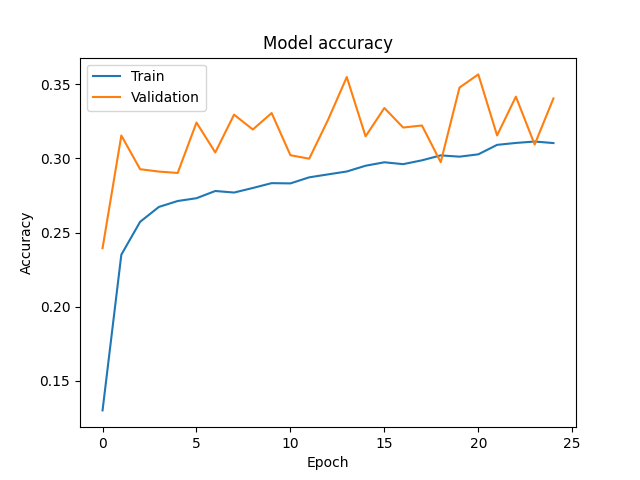
\includegraphics[width=\linewidth]{images/acc_bach_big_categorical_crossentropy_Nadam_sigmoid_n86_tps8_ws96.png}
    \caption{Accuracy plotted over epochs during training.}
    \label{fig:acc}
\end{figure}

\subsection{Generation}
% Explain LSTM gen (jorn)
The output of our model can not be used directly to generate music, as the model will always learn that the most reliable prediction is to repeat the last note. Thus, if the song is generated by using a softmax or by applying a threshold to the output, the result will almost always be a single constant note. Instead, we treat the output as a probability vector, which is used to select a number of notes.

At the start of the generation process, an output buffer is initialized, of which the first \texttt{window\_size} elements are copied from the end of the input data. Then, the following happens for each to be generated tick:

\paragraph{Model output} The preceding \texttt{window\_size} elements are fed into the network to create the output $Y$. 

\paragraph{Candidate notes} The number of potential (or candidate) notes $c$ is estimated using \autoref{eqn:candidates}, by counting the number of elements that are relatively probable to be selected.

\begin{equation}\label{eqn:candidates}
    c = \lvert \{ y \in Y : y > \max(Y) - 2\sigma(Y) \} \rvert
\end{equation}


\paragraph{Number of active notes} The number of active notes $n$ is computed by taking the mean of $c$, the value of $n$ for the previous tick and the mean value for $n$ in the input data. Additionally, $n$ may never be greater than the greatest value for $n$ in the input data. This is done to prevent sudden changes to the number of active notes.

\paragraph{Threshold} All values smaller than 0.5\% of the maximum value in $Y$ are set to 0, to prevent them from being chosen.

\paragraph{Encourage repeating notes} The original model behavior of repeating the last note is desirable to a certain degree. To make that outcome more likely, the probability for the notes active in the previous step is doubled.

\paragraph{Choose notes} Finally, $Y$ is normalized and used as a probability vector to randomly choose $n$ notes to make active in the current step.

\mbox{} % add a bit of vertical space

When all notes are generated, a few post-processing operations are applied. The original input data is removed from the result, and if there is a window in the result where the notes are unchanged (which results in a period of silence), that is considered the end of the song. 

Additionally, notes that were only active for a single tick before being deactivated again are removed from the result. While such behavior is quite possible in normal music, we found that their presence made the result sound more erratic than desired. 



\section{Results}
\label{sec:results}
The accuracy achieved after different training configurations are shown in \autoref{tab:results}. From the table we can see that the accuracy measures of the test accuracy after 25 epochs or after the validation loss stops improving. Here, activation refers only to the activation of the output layer. The cells which are highlighted in the table represent changes from previous best configuration.

We have also plotted a graph representing the accuracy of the model during the training of epochs which can be seen in figure \ref{fig:acc}. We can observe that as the training number of epoch’s increases, the validation accuracy is increased. The categorical cross-entropy which determines the loss over epochs can be seen in figure \ref{fig:loss}. The loss function caused the network to converge much slower but it eventually achieved an accuracy of 29\%.

\subsection{Generated music}
\begin{figure}
    \centering
    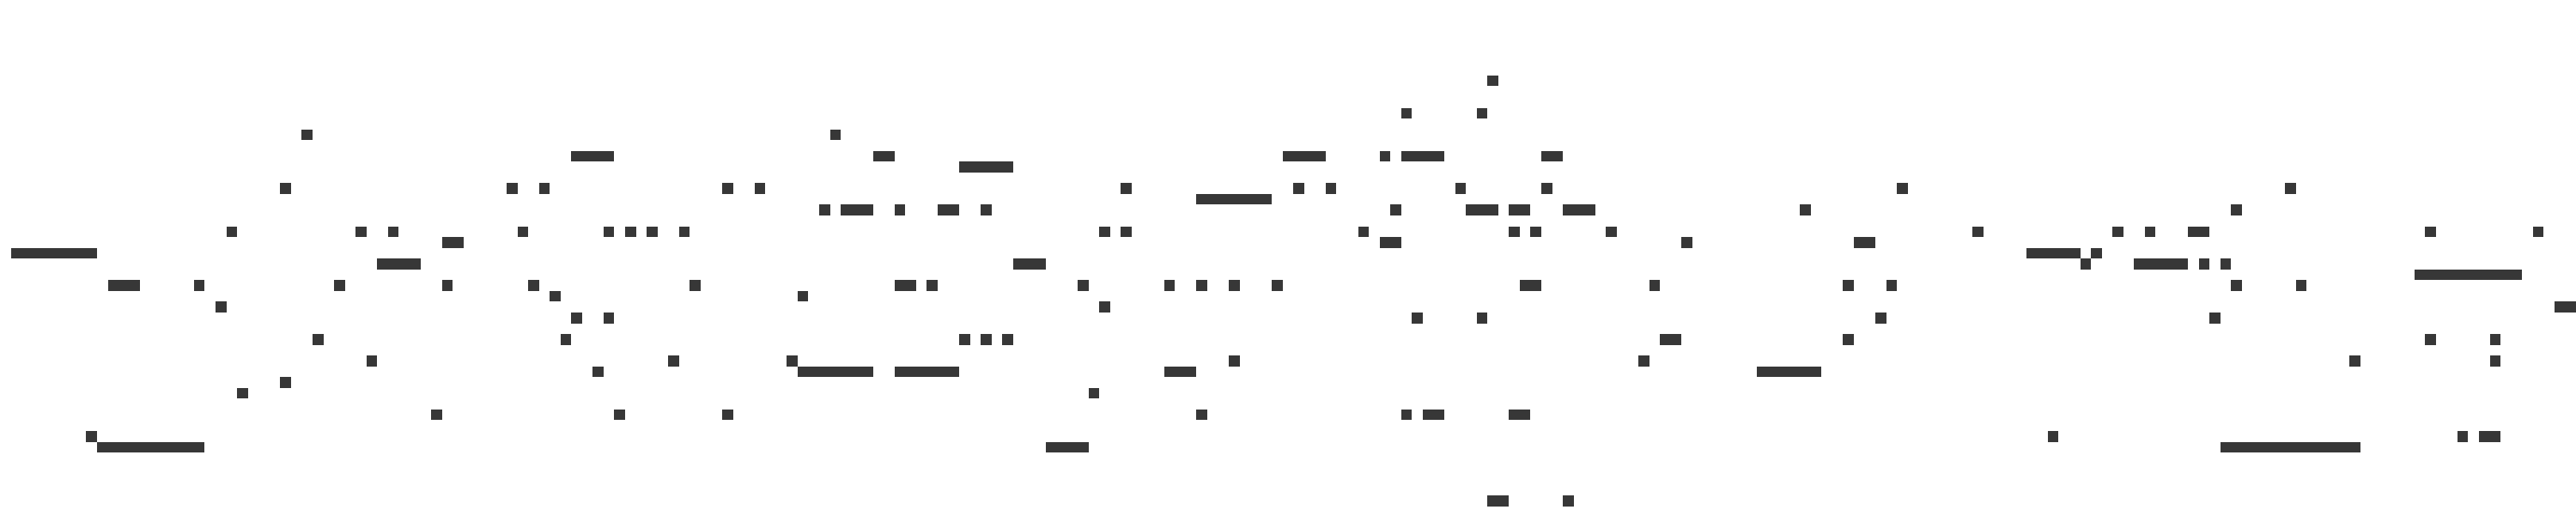
\includegraphics[width=\linewidth]{images/hmm_samples.png}
    \caption{Notes generated by the hidden Markov model. The vertical axis represents pitch, the horizontal axis represents time.}
    \label{fig:hmm_samples}
\end{figure}

\begin{figure}
    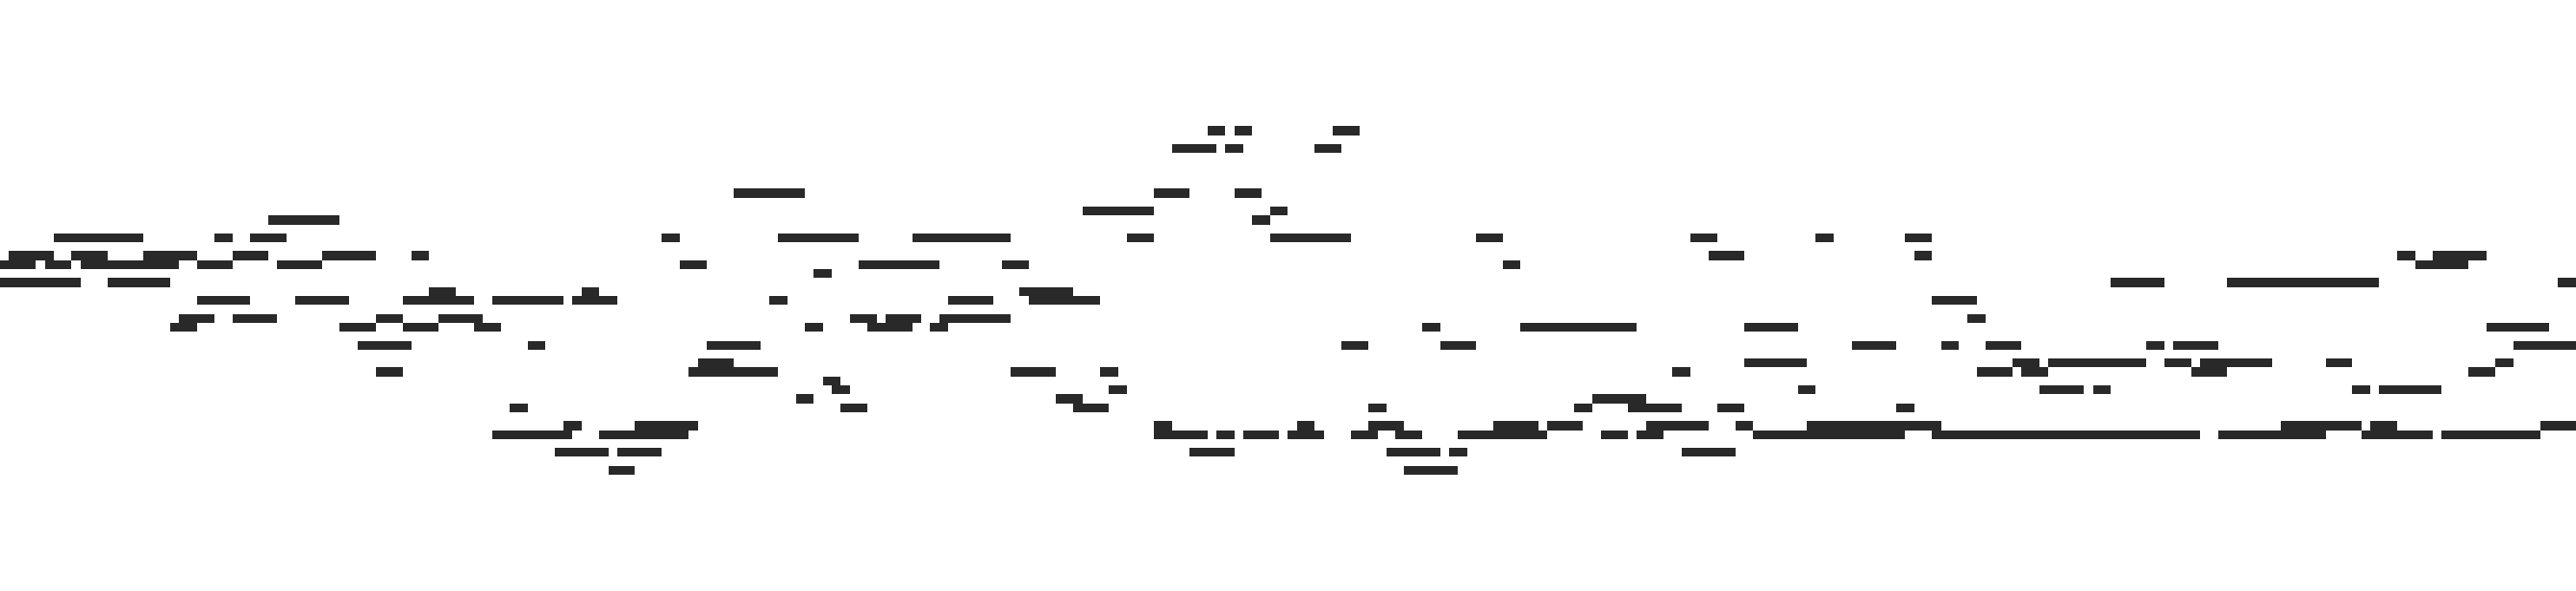
\includegraphics[width=\linewidth]{images/lstm_samples.png}
    \caption{Notes generated by the LSTM model. The vertical axis represents pitch, the horizontal axis represents time.}
    \label{fig:lstm_predicted}
\end{figure}

We used both our Hidden Markov Model (HMM) and LSTM to generated music. An image of music generated by our HMM can found in \autoref{fig:hmm_samples}. The produced result would not fool an expert into thinking this was actually produced by Bach, but there is some musical structure to it. The model often produces notes that are held for only one tick, which does not happen in the input data. 

An example of music generated by our LSTM model can be found in \autoref{fig:lstm_predicted}. Visually, this looks somewhat similar to \autoref{fig:input_samples}, but without the clear separation of the 4 different tracks. The output looks quite a bit cleaner compared to the HMM result, and the same can be said when listening to the music. However, most listeners would still be able to determine that this music was generated by a computer, and not by Bach.


Music generated by the HMM is a bit fast paced and mostly have high and some random notes in it. The music generated by the LSTM has a much better melody and more in sync with the composition. Since HMMs rely on strong assumptions and are much simpler than a recurring neural network, the audio generated by LSTM model is much better.



% This is just for the web version
\ifpdf
Examples of the output for our hidden Markov model and our LSTM model can be found on the online version of this report\footnote{Available online at \url{https://ruurdbijlsma.github.io/bach-ex-machina/}}.
\else
Below you can listen to music generated by our hidden Markov model and our LSTM model. The LSTM model is only trained on Bach's music, so it can only predict Bach's music. The hidden Markov model uses only the start of the input song to predict the ending of it, meaning it can predict the ending of any song, albeit only a piano version.

Original: Bach - The Art of Fugue (unfinished):

startaudio midi/unfinpiano.wav endaudio

Generated audio using a hidden Markov model, creating and ending for Bach - The Art of Fugue:

startaudio midi/unfinpredicted.wav endaudio

Generated audio using our LSTM model, creating and ending for Bach - The Art of Fugue:

startaudio midi/lstmunfin.wav endaudio

Original: Toto - Africa (piano version):

startaudio midi/africapiano.wav endaudio

Generated audio using a hidden Markov model, based on Toto - Africa:

startaudio midi/africapredicted.wav endaudio

\fi

\section{Discussion}
 We trained a deep LSTM sequential prediction model and have successfully got the model to learn musical concepts without any prior knowledge or supervision from experts.

From the results, we can comfortably claim that we have accomplished what we aimed for in our research. We have built a model that is capable of autonomously generating the ending of a given classical song. We have successfully trained a time-series model using a dataset of Bach's compositions. We then implemented this model to finish The Art of Fugue.

We tried various types of loss functions and many variations in the architecture to build the best model we can (as discussed in Section \ref{architecture}). The output generated by the model has a good musical structure and does fit in well as a continuation of the unfinished composition. However, one can clearly tell the difference between Bach's style of composition and the music generated by the model.

This implementation may be further improved by trying out different input encodings that might be better suited for the network. Another approach possible approach would be to use the 4 tracks of Bach's unfinished fugue separately for training the network instead of using them all combined.

\bibliographystyle{plain}
\bibliography{references}


\end{document}


